\chapter{Statistical Analysis and Graphing Techniques}
\pagestyle{fancy}
\fancyhf{}
\fancyhead[OC]{\leftmark}
\fancyhead[EC]{\rightmark}
%\renewcommand{\footrulewidth}{1pt}
\cfoot{\thepage}

\section{Key Concepts and Formulae}
\begin{enumerate}
    \item Often, it is easier and useful to plot the data by linearizing the equation or expression related to the data. Taking 'ln' on both sides, is one of the ways to linearize the equation of higher degree polynomials. For instance, PV$^\gamma$ = const. Taking 'ln' on both sides, we get: lnP + $\gamma$lnV = ln(const.). 
    \item least square fit: While tracing the curve along the points in the graph, trace such that the points are equally distributed around the curve. That is the sum of the square of the distance between the points and the curve should be minimum. 
    \item Students should take care of following things to get the maximum possible points in the olympiad exams.\\
    a) Make sure you have a well defined table of data with correct values of each parameter. \\
    b) Use at least 80 percent of the graph paper. Do not make a small graph and leave the rest of the graph paper blank. Do the calculations, if there are any, in a separate page. \\
    c) Label your axes properly and choose an appropriate scale for them.\\
    d) Make your plot as smooth as possible. Using pencil is therefore a good idea!\\
    e) To find the slope from the curve (straight line), take points that are considerably far. 
\end{enumerate}
\section{Level 1 Problems and Solutions}
\begin{enumerate}
    \item A lab worker makes measurement of the temperature and pressure of an ideal gas during the adiabatic process. The results, in terms of T$_0$ and V$_0$ are:
\begin{center}
\begin{tabular}{|c|c|c|c|c|c|c|c|c|} 
 \hline
 pressure & units of P$_o$ & 1.21& 1.41& 1.59&1.73&2.14 \\ 
 \hline
 temperature & units of T$_o$ & 2.11 &2.21 &2.28 &2.34 &2.49\\ 
 \hline
\end{tabular}
\end{center}
Plot an appropriate graph from this data that can be used to determine the adiabatic constant $\gamma$.
\item A student obtains the following readings in volt and milliampere for the connections to the black box.
\begin{center}
\begin{tabular}{ |c|c|} 
  \hline
 V\text{(V)}& I\text{(mA)}\\
 \hline
 0.53& 0.54 \\
 \hline
 0.77 &0.77 \\
 \hline
 1.02 &1.01\\
 \hline
 1.49 &1.51 \\
 \hline
 1.98& 2.02 \\
 \hline
 2.49 &2.51 \\
 \hline
\end{tabular}
\end{center}
In each case plot V (on Y-axis)-I (on X-axis) on the graph papers provided. Preferably use a pencil to plot. Calculate the value of resistance from the plot. Show your calculation. \\
\item While performing an experiment with a liquid z (specific heat capacity 2.19kJ Kg K$^{-1}$), an experimenter starts with 200 ml of the liquid z in a beaker on a hot plate which is attached with scales to measure mass on it along with time. There is no lid over the beaker and the liquid is kept exposed to the surrounding. The experimenter inserts a thermometer such that it is always in contact with the liquid near the bottom of the beaker. The experimenter turns on the hot plate at t=0 min. and records the liquid temperature as well as the combined mass of the liquid, beaker and thermometer every minute. After 24 mins, he observes that there is no more liquid in the beaker. The observations are tabulated below: \\
\begin{center}
\begin{tabular}{ |c|c|c|c|c|c|c|c|c|c|c|c|} 
 \hline
 Time(mins) & 0 &1 &2 &3 &4 &5 &6 &7 &8 &9 &10 \\ 
 \hline
 temp($\degree$C) &24 &25 &28 &37 &50 &64 &77 &90 &102 &113 &124\\ 
 \hline
 Mass(gm)&310 &310 &310 &310 &310 &310 &310 &310 &310 &310 &310\\
 \hline
\end{tabular}
\end{center}

\begin{center}
\begin{tabular}{ |c|c|c|c|c|c|c|c|c|c|c|c|c|c| } 
 \hline
 11& 12& 13 &14 &15 &16 &17 &18 &19 &20 &21 &22 &23 &24 \\
 \hline
 134 &143 &152 &158 &160 &160 &160 &159 &160 &160 &161 &160 &161 &- \\
 \hline
 307 &307 &305 &302 &288 &264 &241 &214 &190 &165 &138 &110 &79 &69\\
 \hline
\end{tabular}
\end{center}
Based on the above data
\begin{enumerate}
    \item Plot a qualitative graph between the rate of change of temperature vs. temperature i.e. $\Delta$T/$\Delta$t vs T. (Make an appropriate Table for the plot)
    
    \item Identify the temperature T at which dT/dt becomes zero. 
    
    \item From(b) which intrinsic property of the liquid can be inferred ? What is the value? 
    
    \item Give two possible reasons as to why the there is a 1$\degree$ fluctuation in temperature after 15 mins.
    
    \item Plot m vs. t after t = 15 min.
\end{enumerate}
\textbf{Hints and Solution:}\\\\
a) For making an appropriate table for the plot, we need: \\
\[\text{t(min), which is already given.}\]
\begin{align*}
    T &= \dfrac{T_1 + T_2}{2} \degree C\\ 
    \Delta T &= T_2 - T_1 \degree C\\
    \Delta t &= t_2 - t_1 (min)\\
    \Delta T/\Delta t 
\end{align*}
The graph should look something like this: 
\textbf{\begin{figure}[htp]
    \centering
    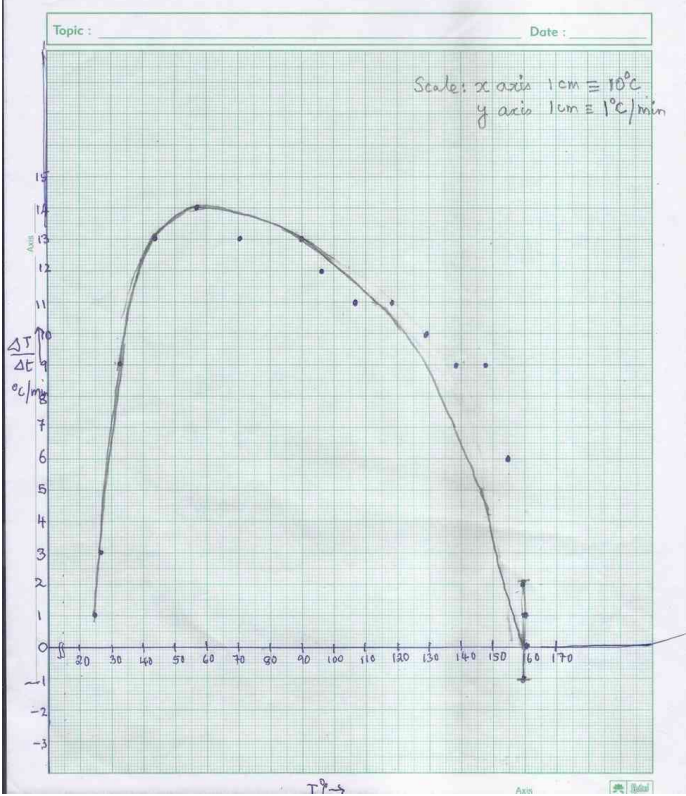
\includegraphics[width=17cm, scale=1.5]{mainmatter/graph1.PNG}
    \caption{}
    \label{fig:thermo3.5}
\end{figure}} \clearpage
b) T = 160$\degree$C\\
c) Intrinsic property = Boiling Point, and value = 160$\degree$C\\
d) The graph should look like this:\\
\textbf{\begin{figure}[htp]
    \centering
    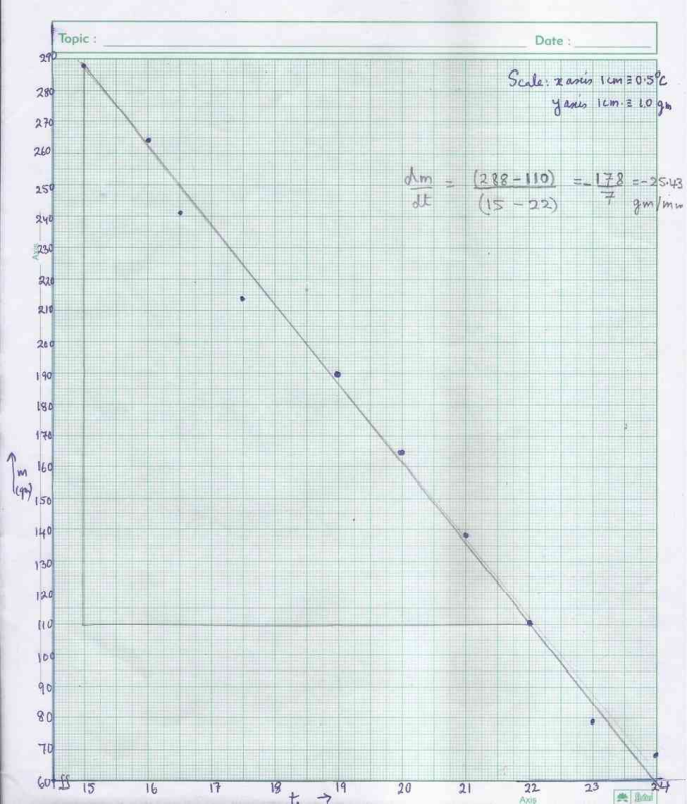
\includegraphics[width=15cm, scale=1.5]{mainmatter/graph2.PNG}
    \caption{}
    \label{fig:thermo3.5}
\end{figure}} \clearpage
\end{enumerate}